%% This is file `prletters-template.tex',
%%
%% Copyright 2013 Elsevier Ltd
%%
%% This file is part of the 'Elsarticle Bundle'.
%% ---------------------------------------------
%%
%% It may be distributed under the conditions of the LaTeX Project Public
%% License, either version 1.2 of this license or (at your option) any
%% later version.  The latest version of this license is in
%%    http://www.latex-project.org/lppl.txt
%% and version 1.2 or later is part of all distributions of LaTeX
%% version 1999/12/01 or later.
%%
%% The list of all files belonging to the 'Elsarticle Bundle' is
%% given in the file `manifest.txt'.
%%
%% Template article for Elsevier's document class `elsarticle'
%% with harvard style bibliographic references
%%
%% $Id: prletters-template-with-authorship.tex 69 2013-07-15 10:15:25Z rishi $
%%
%% This template has no review option
%%
%% Use the options `twocolumn,final' to obtain the final layout
\documentclass[times,twocolumn,final,authoryear]{elsarticle}

%% Stylefile to load PR Letters template
\usepackage{prletters}
\usepackage{framed,multirow}

%% The amssymb package provides various useful mathematical symbols
\usepackage{amssymb}
\usepackage{latexsym}

% Following three lines are needed for this document.
% If you are not loading colors or url, then these are
% not required.
\usepackage{url}
\usepackage{xcolor}

\usepackage{natbib}
\usepackage{bbm}
\usepackage{amssymb}
\usepackage{amsmath,amsfonts,amsthm}
\usepackage{graphicx}
\usepackage{caption}
\usepackage{subfigure}
\usepackage{subfig}
\newcommand{\mrsid}{{\sc \texttt{Mr}.~\texttt{Sid}}}
\providecommand{\mb}[1]{\boldsymbol{#1}}
\newcommand{\bx}{\mb{x}}
\newcommand{\by}{\mb{y}}
\newcommand{\bX}{\mb{X}}
\newcommand{\bY}{\mb{Y}}
\newcommand{\T}{^{\ensuremath{\mathsf{T}}}}           % transpose
\newcommand{\argmax}{\operatornamewithlimits{argmax}}
\newcommand{\argmin}{\operatornamewithlimits{argmin}}
\newcommand{\diag}{\operatornamewithlimits{diag}}
\let\oldref\ref
\renewcommand{\ref}[1]{(\oldref{#1})}

\definecolor{newcolor}{rgb}{.8,.349,.1}
\journal{Pattern Recognition Letters}

\begin{document}

\thispagestyle{empty}

\begin{table*}[!th]

\begin{minipage}{.9\textwidth}
\baselineskip12pt
\ifpreprint
  \vspace*{1pc}
\else
  \vspace*{-6pc}
\fi

\noindent {\LARGE\itshape Pattern Recognition Letters}
\vskip6pt

\noindent {\Large\bfseries Authorship Confirmation}

\vskip1pc


{\bf Please save a copy of this file, complete and upload as the
``Confirmation of Authorship'' file.}

\vskip1pc

As corresponding author
I, \underline{  Shaojie Chen  }, hereby confirm on behalf of all authors that:

\vskip1pc

\begin{enumerate}
\itemsep=3pt
\item This manuscript, or a large part of it, \underline {has not been
published,  was not, and is not being submitted to} any other journal.

\item If \underline {presented} at or \underline {submitted} to or
\underline  {published }at a conference(s), the conference(s) is (are)
identified and  substantial \underline {justification for
re-publication} is presented  below. A \underline {copy of
conference paper(s) }is(are) uploaded with the  manuscript.

\item If the manuscript appears as a preprint anywhere on the web, e.g.
arXiv,  etc., it is identified below. The \underline {preprint should
include a  statement that the paper is under consideration at Pattern
Recognition  Letters}.

\item All text and graphics, except for those marked with sources, are
\underline  {original works} of the authors, and all necessary
permissions for  publication were secured prior to submission of the
manuscript.

\item All authors each made a significant contribution to the research
reported  and have \underline {read} and \underline {approved} the
submitted  manuscript.
\end{enumerate}

Signature\underline{  Shaojie Chen  } Date: \underline{  07/17/2016  }
\vskip1pc

\rule{\textwidth}{2pt}
\vskip1pc

{\bf List any pre-prints:}
arXiv
\vskip5pc


\rule{\textwidth}{2pt}
\vskip1pc

{\bf Relevant Conference publication(s) (submitted, accepted, or published):}
Not available
\vskip5pc



{\bf Justification for re-publication: }
Not available
\end{minipage}
\end{table*}

\clearpage
\thispagestyle{empty}
\ifpreprint
  \vspace*{-1pc}
\fi

\begin{table*}[!th]
\ifpreprint\else\vspace*{-5pc}\fi

\section*{Research Highlights}

\vskip1pc

\fboxsep=6pt
\fbox{
\begin{minipage}{.95\textwidth}
\vskip1pc
\begin{itemize}

 \item The proposed model generalizes the traditional linear dynamical system model

 \item An efficient algorithm is designed for parameter estimation

 \item The model works very well on high-dimensional neuro-imaging data

 \item It is also a standard tool for big time-series data analysis in many domains

\end{itemize}
\vskip1pc
\end{minipage}
}

\end{table*}

\clearpage


\ifpreprint
  \setcounter{page}{1}
\else
  \setcounter{page}{1}
\fi

\begin{frontmatter}

\title{An M-Estimator for Reduced-Rank System Identification}

\author[a]{Shaojie \snm{Chen} \corref{cor1}}
\cortext[cor1]{Corresponding author:+1-410-409-8132; pzcsj76@gmail.com}
\author[b]{Kai \snm{Liu}}
\author[c]{Yuguang \snm{Yang}}
\author[a]{Yuting \snm{Xu}}
\author[d]{Seonjoo \snm{Lee}}
\author[a]{Martin \snm{Lindquist}}
\author[a]{Brian S. \snm{Caffo}}
\author[e,f]{Joshua T. \snm{Vogelstein}}
\address[a]{\small Dept. of Biostatistics, Johns Hopkins Bloomberg School of Public Health, Baltimore 21205, USA}
\address[b]{Dept. of Neuroscience, Johns Hopkins University, Baltimore 21205, USA}
\address[c]{Dept. of Chemical and Biomolecular Engineering, Johns Hopkins University, Baltimore 21205, USA}
\address[d]{Dept. of Psychiatry and Department of Biostatistics, Columbia University, New York City 10027, USA}
\address[e]{Child Mind Institute, Baltimore 21205, USA}
\address[f]{Dept. of Biomedical Engineering and Institute for Computational Medicine, Johns Hopkins University, Baltimore 21205, USA}

\received{1 May 2013}
\finalform{10 May 2013}
\accepted{13 May 2013}
\availableonline{15 May 2013}
\communicated{S. Sarkar}


\begin{abstract}
High-dimensional time-series data from a wide variety of domains, such as neuroscience, are being generated every day. Fitting statistical models to such data, to enable parameter estimation and time-series prediction, is an important computational primitive. Existing methods, however, are unable to cope with the high-dimensional nature of these data, due to both computational and statistical reasons.  We mitigate both kinds of issues by proposing an M-estimator for Reduced-rank System IDentification (\mrsid). A combination of low-rank approximations, $\ell_1$ and $\ell_2$ penalties, and some numerical linear algebra tricks, yields an estimator that is computationally efficient and numerically stable.  Simulations and real data examples demonstrate the usefulness of this approach in a variety of problems.  In particular, we demonstrate that \mrsid~can accurately estimate spatial filters, connectivity graphs, and time-courses from native resolution functional magnetic resonance imaging data. \mrsid~therefore enables big time-series data to be analyzed using standard methods, readying the field for further generalizations including nonlinear and non-Gaussian state-space models.
\end{abstract}

\begin{keyword}
%\MSC 41A05\sep 41A10\sep 65D05\sep 65D17
%\KWD Keyword1\sep Keyword2\sep Keyword3
 high dimension\sep image processing\sep parameter estimation \sep state-space model \sep time series analysis
%% MSC codes here, in the form: \MSC code \sep code
%% or \MSC[2008] code \sep code (2000 is the default)
\end{keyword}

\end{frontmatter}

%\linenumbers

%% main text
\section{Introduction}
High-dimensional  time-series data are becoming increasingly  abundant across a wide variety of domains, spanning economics \citep{Johansen1988}, neuroscience \citep{Friston2003a},   and cosmology \citep{Xie2013a}. Fitting statistical models to such data, to enable parameter estimation and time-series prediction, is an important computational primitive.
Linear dynamical system (LDS) models are amongst the most popular and powerful, because of their intuitive nature and ease of implementation \citep{Kalman1963}.   The famous Kalman Filter-Smoother is one of the most popular and powerful tools for time-series prediction with an LDS, given known parameters \citep{Kalman1960a}.

In practice, however, for many LDS's, the parameters are unknown and must be estimated in a process often called \emph{system identification} \citep{Ljung1998}.  To the best of our knowledge, currently there does not exist a methodology that provides parameter estimates and predictions for ultra-high-dimensional time-series data (e.g. the dimension of the time series, $p > 10$,$000$).

The challenges associated with high-dimensional time-series estimation and prediction are multifold.  First, na\"ively, such models include dense $p \times p$ matrices, which are often too large to store, much less invert in memory.  Several recent efforts to invert large sparse matrices using a series of computational tricks show promise, though they are still extremely computationally expensive  \citep{Hsieh2013, Banerjee2013a}.

Second, estimators behave poorly due to numerical instability.
Reduced-rank LDS models can partially address this problem by reducing the number of latent states.  \citep{CHEN1989}.  However, without further constraints, the dimensionality of the latent states would be reduced to such an extent  that it would significantly decrease the predictive capacity of the resulting model.  Third, even after addressing these problems, the time to compute all the necessary quantities can be overly burdensome. Distributed memory implementations, such as those built with Spark, might help overcome this problem. However, it would lead to additional costs and set-up burden, as it would require a Spark cluster \citep{Zaharia2010}.

We address all three of these issues with our M-estimator for Reduced-rank  System IDentification (\mrsid).  By assuming the dimensionality of the latent state space is small (i.e. reduced-rank), relative to the observed space dimensionality, we can significantly improve computational tractability and estimation accuracy. By further penalizing the estimators, with $\ell_1$ and/or $\ell_2$ penalties, via utilizing prior knowledge on the structure of the parameters, we gain further estimation accuracy in this high-dimensional but relatively low-sample size regime.  Finally, by employing several numerical linear algebra tricks, we can reduce the computational burden significantly.

These three techniques combined enable us to obtain highly accurate estimates in a variety of simulation settings.  \mrsid~is, in fact, a generalization of the now classic Baum-Welch expectation maximization algorithm, commonly used for system identification in much lower dimensional linear dynamical systems \citep{rabiner1989tutorial}. We show numerically that the hyperparameters can be selected to minimize prediction error on held-out data.  Finally, we use \mrsid~to estimate functional connectomes from the motor cortex.  \mrsid~enables us to estimate the regions, rather than imposing some prior parcellation on the data, as well as estimate sparse connectivity between regions.  \mrsid~reliably estimates these connectomes, as well as predicts the held-out time-series data.  To our knowledge, this is the first time a single unified approach has been used to estimate partitions and functional connectomes directly from the high-dimensional data.

This work presents a new analysis of a model which has only been implemented in low-dimensional settings,
and paves the way for high-dimensional implementation. Though primitive, it is a first step for essentially any high-dimensional time series analysis, control system identification, and spatiotemporal analysis. To enable extensions, generalizations, and additional applications, the code for the core functions and generating each of the figures is freely available on Github (\url{https://github.com/shachen/PLDS/}).

\section{The Model}
In statistical data analysis, one often encounters some observed variables, as well as some unobserved latent variables, which we denote as $\bY=(\by_1,\ldots,\by_T)$ and $\bX=(\bx_1,\ldots,\bx_T)$ respectively. By the Bayes rule, the joint probability of $\bX$ and $\bY$ is $P(\bX,\bY)=P(\bY|\bX) P(\bX)$. The conditional distribution $P(\mb{Y}|\mb{X})$ and prior $P(\mb{X})$ can both be represented as a product of marginals:

\begin{equation*}
\begin{aligned}
P(\mb{Y}|\mb{X}) &= \prod_{t=1}^T P(\by_t | \by_0,\ldots,\by_{t-1}, \bx_0,\ldots,\bx_{t-1}), \\
P(\bX) &= P(\bx_0) \prod_{t=1}^T P(\bx_t | \bx_0,\ldots,\bx_{t-1}).
\end{aligned}
\end{equation*}

The generic time-invariant state-space model (SSM) makes the following simplifying assumptions:
\begin{equation}
\label{eq:genericssm}
\begin{aligned}
P(\by_t | \by_0,\ldots,\by_{t-1}, \bx_0,\ldots,\bx_t)  &\approx P(\by_t | \bx_t), \\
P(\bx_t | \bx_0,\ldots,\bx_{t-1}) &\approx P(\bx_t | \bx_{t-1}).
\end{aligned}
\end{equation}

A linear dynamical system (LDS) further assumes that both terms in \ref{eq:genericssm} are linear Gaussian functions, which when written as an iterative random process, yield the standard matrix update rules:
\begin{equation*}
\begin{aligned}
&\bx_{t+1}=A\bx_t+\mathbf{w}_t, \quad \mathbf{w}_t\sim N(\mathbf{0},Q),\quad \bx_0 \sim N(\mathbf{\pi}_0,V_0), \\
&\by_t=C\bx_t+\mathbf{v}_t,\qquad \mathbf{v}_t\sim N(\mathbf{0},R),
\end{aligned}
\end{equation*}
where $A$ is a $d\times d$ state transition matrix and $C$ is a $p \times d$ generative matrix. $\bx_t$ is a $d\times 1$ vector and $\by_t$ is a $p\times 1$ vector.
% The sequence of vectors $\bY=(\by_1,\ldots,\by_T)$ are the observed data and $\bX=(\bx_1,\ldots,\bx_T)$ represent the unknown hidden states.
The output noise covariance $R$ is $p\times p$, while the state noise covariance $Q$ is $d\times d$. Initial state mean $\mathbf{\pi}_0$ is $d\times 1$ and covariance $V_0$ is $d \times d$.

The model can be thought of as a continuous version of the hidden Markov model (HMM), where the columns of $C$ stand for the hidden states and one observes a single state at time $t$. Unlike HMM, LDS \ref{eq:genericssm} allows one to observe a linear combination of multiple states. $A$ is the analogy of the state transition matrix, which describes how the weights $\bx_t$ evolve over time. Another difference is that LDS contains two white noise terms, which are captured by the $Q$ and $R$ matrices.

Without applying further constraints, the LDS model itself is unidentifiable. Three minimal constraints are introduced for identifiability:
\vspace*{-1mm}
\begin{flalign*}
&\text{Constraint 1: }Q \text{ is the identity matrix}\\
&\text{\text{Constraint 2:} the order of } C \text{'s columns is fixed based on their norms}\\
&\text{Constraint 3: } V_0=\mathbf{0} &
\end{flalign*}
Note that the first two constraints follow directly from Roweis and Ghahramani (1999), which try to eliminate the degeneracy in the model. Additionally, $V_0$ is set to zero, meaning the starting state $\bx_0=\mathbf{\pi}_0$ is an unknown constant instead of a random variable. We put this constraint on, because in the application that follows only one single chain of time series observed. To estimate $V_0$, multiple series of observations are required.

The following three constraints are further applied to achieve a more useful model:
\vspace*{-1mm}
\begin{flalign*}\label{eqn:constraints2}
&\text{Constraint 4: }R\text{ is a diagonal matrix} \\
&\text{Constraint 5: }A\text{ is sparse}\\
&\text{Constraint 6: }C\text{ has smooth columns} &
\end{flalign*}

The constraint on $R$ is natural. Consider the case where the observatons are high dimensional, which means that the  $R$ matrix is very large. One cannot accurately estimate the many free parameters in $R$ with a limited amount of observations. Therefore, some constraints on $R$ will help with inferential accuracy, by virtue of significantly reducing variance while not adding too much bias. For example, $R$ can be set to multiples of the identity matrix, or more generally, a diagonal matrix. A static LDS model with a diagonal $R$ is equivalent to Factor Analysis, while one with multiples of the identity $R$ matrix leads to Principal Component Analysis (PCA) \citep{roweis1999unifying}.

The $A$ matrix is the transition matrix of the hidden states. In many applications, it is desirable for $A$ to be sparse. An $\ell_1$ penalty on $A$ is used to impose the sparsity constraint. In the applications that follow, $A$ is a central construct of interest representing a so-called connectivity graph, and the graph is expected to be sparse.

Similarly, in many applications, it is desirable for the columns of $C$ to be smooth. For example, in neuroimaging data analysis, each column of $C$ can be a signal in the brain. Having the signals spatially smooth can help extract meaningful information from the noisy neuroimaging data. In this context, an $\ell_2$ penalty on columns of $C$ is used to enforce smoothness.

With all those constraints, the model becomes:
\begin{equation}\label{eq:model0}
\begin{aligned}
	&\bx_{t+1}=A\bx_{t}+\mathbf{w}_t, \quad \mathbf{w}_t\sim N(\mathbf{0},\mathbf{I}),\quad \bx_0 = \mathbf{\pi}_0,\\
	&\by_t=C\bx_t+\mathbf{v}_t,\qquad \mathbf{v}_t\sim N(\mathbf{0},R),
\end{aligned}
\end{equation}
where $A$ is a sparse matrix and $C$ has smooth columns.

Let $\theta =\{A,C,R,\mathbf{\pi}_0\}$ represent all unknown parameters, while $P(\bX,\bY)$ represents the full likelihood. Then, combining model \ref{eq:model0} and the constraints on $A$ and $C$ leads us to an optimization problem:
\begin{equation}\label{eqn:penaltylik}
\hat{\theta}=\argmin_{\substack{\theta}}\left\{-\log P_\theta(\bX,\bY)+\lambda_1\|A\|_1+\lambda_2\|C\|_2^2\right\}
\end{equation}
where $\lambda_1$ and $\lambda_2$ are tuning parameters and $\|\centerdot\|_p$ represents the $p$-norm of a vector. Equivalently, this problem has the following dual form:
\begin{equation*}\label{eqn:penaltylikdual}
\begin{aligned}
&\text{minimize}&\left\{-\log P_\theta(\bX,\bY)\right\}&\\
&\text{subject to: }
& \alpha\|A\|_1+ (1-\alpha)\|C\|_2^2 \leq \varphi \text{ for some }\varphi; &\\
&& A\in \mathcal{A}_{d\times d},\ C \in \mathcal{C}_{p \times d}, R \in \mathcal{R}_{p\times p}, \pi_0 \in \mathcal{\pi}_{d\times 1}&
\end{aligned}
\end{equation*}
where $\alpha = \frac{\lambda_1}{\lambda_1 + \lambda_2}$. $\mathcal{A}_{d\times d}$ and $\mathcal{C}_{p \times d}$ are $d\times d$ and $p \times d$ dimensional matrix spaces respectively. $\mathcal{R}_{p \times p}$ is the $p \times p$ diagonal matrix space and $\mathcal{\pi}_{d\times 1}$ is the $d$ dimensional vector space.
\section{Parameter Estimation}
Replacing $\log  P(\bX,\bY)$ in problem \ref{eqn:penaltylik} with its concrete form, one gets
\begin{equation}\label{eqn:penaltylik2}
\begin{split}
\hat{\theta}=\argmin_{\substack{\theta}}\biggl\{&\sum\limits_{t=1}^{T}\big(\frac{1}{2}[\by_t-C\bx_t]^{\T}R^{-1}[\by_t-C\bx_t]\big)-\frac{T}{2}\text{log}|R|\\
&+\sum\limits_{t=1}^{T}\big(\frac{1}{2}[\bx_t-A\bx_{t-1}]^{\T}[\bx_t-A\bx_{t-1}]\big)-\frac{T}{2}\text{log}|\mathbf{I}|\\
&- \text{log}(\mathbbm{1}_{\mathbf{\pi}_0}(\bx_0))+\lambda_1\|A\|_1+\lambda_2\|C\|_2^2\biggr\}\\
\end{split}
\end{equation}

Denote the target function in the curly braces as $\mathbf{\Phi}(\theta,\bY,\bX)$. Then a parameter estimation algorithm is one that optimizes $\mathbf{\Phi}(\theta,\bY,\bX)$ with regard to $\theta=\{A,C,R,\mathbf{\pi}_0\}$.

Parameter estimation for LDS has been investigated extensively in statistics, machine learning, control theory, and signal processing research. For example, in machine learning, the exact and variational inference algorithms for general Bayesian networks can be applied to LDS. In control theory, the corresponding area of study is known as system identification.

Specifically, one way to search for the maximum likelihood estimation (MLE) is through iterative methods such as Expectation-Maximization (EM) \citep{shumway1982approach}. The EM algorithm for a standard LDS is detailed in Zoubin and Geoffrey (1996) \citep{ghahramani1996parameter}. An alternative is to use subspace identification methods such as N4SID and PCA-ID, which give asymptotically unbiased closed-form solutions \citep{van1994n4sid,doretto2003dynamic}. In practice, determining an initial solution with subspace identification and then refining it with EM is an effective approach \citep{boots2009learning}.

However, the above approaches are not directly applicable to optimization problem \ref{eqn:penaltylik} due to the introduced penalty terms. We therefore developed an algorithm called M-estimation for Reduced-rank System IDentification (\mrsid), as described below. \mrsid\  is a generalized Expectation-Maximization (EM) algorithm.

\subsection{E Step}
The E step of EM requires computation of the expected log likelihood, $\Gamma = E[\log P(\bX,\bY)|\bY]$. This quantity depends on three expectations: $E[\bx_t|\bY]$, $E[\bx_t\bx_t^{\T}|\bY]$ and $E[\bx_t\bx_{t-1}^{\T}|\bY]$. For simplicity, we denote their finite sample estimators by:
\begin{equation}\label{eq:expecs}
%\begin{aligned}
\hat{\bx}_t \equiv E[\mathbf{x_t}|\bY],\  \hat{P}_t  \equiv E[\bx_t\bx_t^{\T}|\bY],\  \hat{P}_{t,t-1}  \equiv E[\bx_t\bx_{t-1}^{\T}|\bY].
%\end{aligned}
\end{equation}

Expectations \ref{eq:expecs} are estimated with a Kalman filter/smoother (KFS), which is detailed in the Appendix. Notice that all expectations are taken with respect to the current estimations of parameters.
\subsection{M Step}
Each of the parameters in $\theta =\{A,C,R,\mathbf{\pi}_0\}$ is estimated by taking the corresponding partial derivatives of $\mathbf{\Phi}(\theta,\bY,\bx)$, setting them to zero, and then solving the equations. The details of derivations can be found in the Appendix.

Let the estimations from the previous step be denoted as $\theta^{\text{old}} =\{A^{\text{old}},C^{\text{old}},R^{\text{old}},\mathbf{\pi}_0^{\text{old}}\}$ and the current estimations as $\theta^{\text{new}} =\{A^{\text{new}},C^{\text{new}},R^{\text{new}},\mathbf{\pi}_0^{\text{new}}\}$. The estimation for the $R$ matrix has a closed form, as follows:
\begin{equation}\label{eq:updateR}
R^{\text{new}} = \diag \biggl\{\frac{1}{T}\sum\limits_{t=1}^{T}(\by_t\by_t^{\T}-C^{\text{new}}\hat{\bx}_t\by_t^{\T})\biggr\}
\end{equation}
where $\diag$ extracts the diagonal of the in-bracket term, as we constrain $R$ to be diagonal in Constraint 4.

The estimation for $\mathbf{\pi}_0$ has a closed form. The relevant term $\log(\mathbbm{1}_{\mathbf{\pi}_0}(\hat{\bx}_0))$ is minimized only when $\mathbf{\pi}_0^{\text{new}} = \hat{\bx}_0$.

The estimation for the $C$ matrix also has a closed form. Using a vectorization trick as in \citet{turlach2005simultaneous}, one can derive $C$'s closed form solution with the Tikhonov regularization \citep{tikhonov1943stability}
\begin{equation}\label{eq:updatec}
C^{\text{new}} =\text{Solve with Tikhonov regularization}
\end{equation}

For matrix $A$, its estimation is similar to that of $C$, but slightly more complex. The complexity is that $A$ does not have a closed form solution due to the $\ell_1$ penalty term. However, it can be solved numerically with a Fast Iterative Shrinkage-Thresholding Algorithm (FISTA) \citep{beck2009fast}. The FISTA algorithm is detailed in the Appendix.

With FISTA, matrix $A$ updates as follows:
\begin{equation}\label{eq:updatea}
A^{\text{new}} = \text{Solve with FISTA}
\end{equation}

The parameters in the EM algorithm are initialized with the singular value decomposition (SVD). In addition, several matrix computation techniques are utilized to make the algorithm highly efficient and scalable. The details can be found in the Appendix. Combining the initialization, E-step, and M-step, a complete EM algorithm for \mrsid~is addressed in Table \oldref{tab:em}.\\
\begin{table}
\captionof{table}{The Complete EM Algorithm}
\label{tab:em}
\begin{tabular}{l}
\hline
\textbf{Algorithm } EM Algorithm for \mrsid\\
\hline
1. Initialize $\theta =\{A,C,R,\mathbf{\pi}_0\}$ with SVD\\

2. While convergence criteria are unmet \\

\textbf{E Step}\\
3. Update the expectations in Eq. \ref{eq:expecs} with the KFS\\
% \hline

\textbf{M Step}\\

4. $R^{\text{new}}=\diag\biggl\{\frac{1}{T}\sum\limits_{t=1}^{T}(\by_t\by_t^{\T}-C^{\text{old}} \hat{\bx}_t\by_t^{\T})\biggr\}$, as in Eq.~\ref{eq:updateR}\\
5. $\mathbf{\pi}_0^{\text{new}}=\hat{\bx}_0$\\
6. Update $C^{\text{new}}$, as in Eq.~\ref{eq:updatec}\\
7. Update $A^{\text{new}}$ with FISTA, as in Eq.~\ref{eq:updatea}\\
% 5. Stop when the difference between the estimations from this step and the previous step\\ $\quad$ is less than the tolerance level, or when the maximum number of iterations is reached.\\
\hline
\end{tabular}
\end{table}

\section{Simulations}
\subsection{Simulation Setup}
\label{sec:simsetup}
Two simulations of different dimensions are performed to demonstrate the parameter estimations, computational efficiency, and predicting ability of \mrsid.
In the low dimensional setting, $p = 300$, $d = 10$, and $T = 100$. $A$ is first generated from a random matrix, then elements with small absolute values are truncated to zero to make it sparse. Afterwards, a multiple of the identity matrix is added to $A$. Finally, $A$ is scaled to make sure its eigenvalues fall within $[-1,1]$, thus avoiding diverging time series. Matrix $C$ is then generated as follows. Each column contains random samples from a standard Gaussian. Then, each column is sorted in ascending order. Covariance $Q$ is the identity matrix and covariance $R$ is a multiple of the identity matrix. Initial state $\mathbf{\pi}_0 = \mathbf{0}$ is a zero vector. Pseudocode for data generation can be found in the Appendix.

In the high-dimensional setting, $p = 10000$, $d = 30$, and $T = 100$. The parameters are generated in the same manner. To evaluate the accuracy of estimations, we elect to define the distance between two matrices $A$ and $B$ as
\begin{equation}\label{eq:distance}
d_{A,B} = \argmin_{P\in P(n)}\left\{\log\bigl[\frac{n}{\text{\footnotesize Trace}(P\times C_{A,B})}\bigr]\right\}
\end{equation}
where $C_{A,B}$ is the correlation matrix between columns of A and B, $P(n)$ is a collection of all the permutation matrices of order n, and $P$ is a permutation matrix.

\begin{figure}
\centering
\subfigure[Low dimensional setting]{%
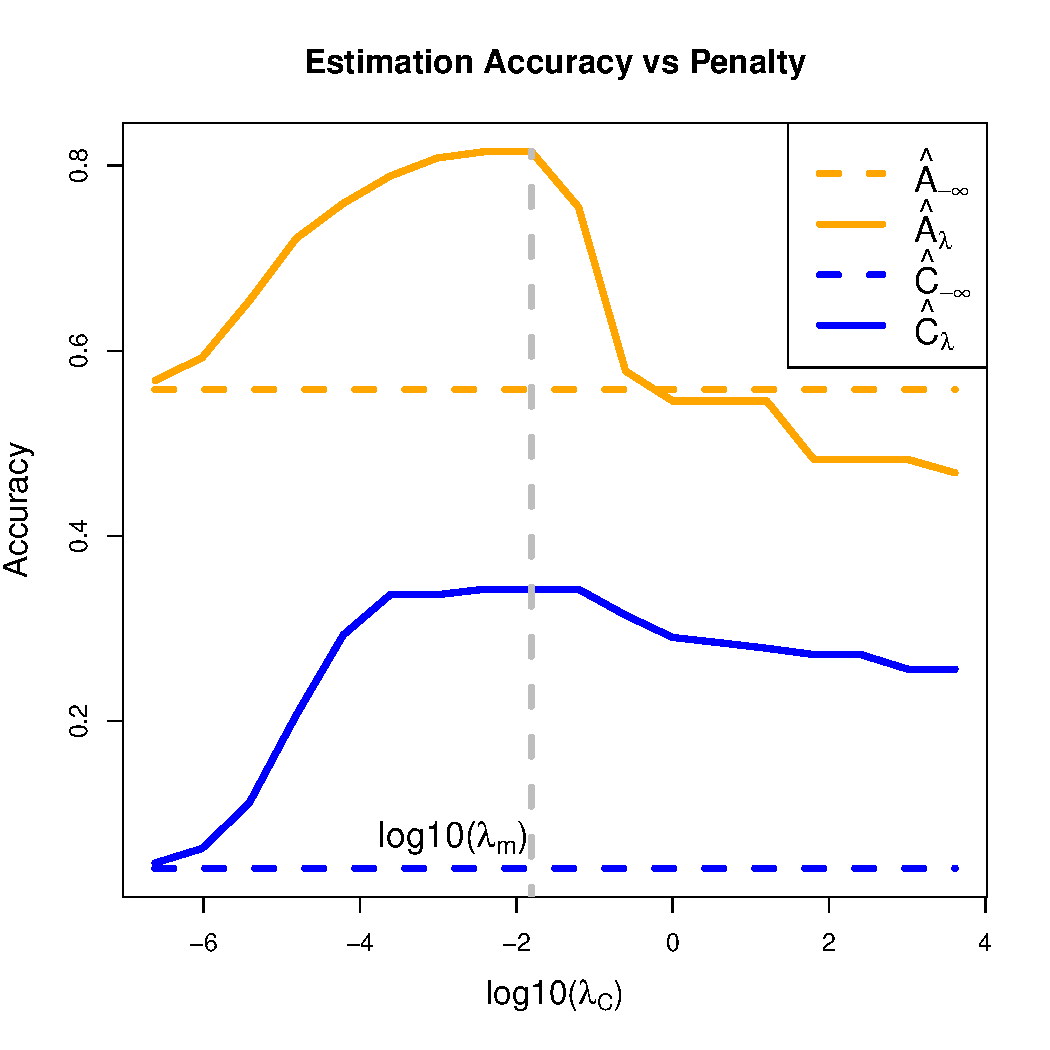
\includegraphics[scale=.43]{low-d-simulation.pdf}
}
\subfigure[High dimensional setting]{%
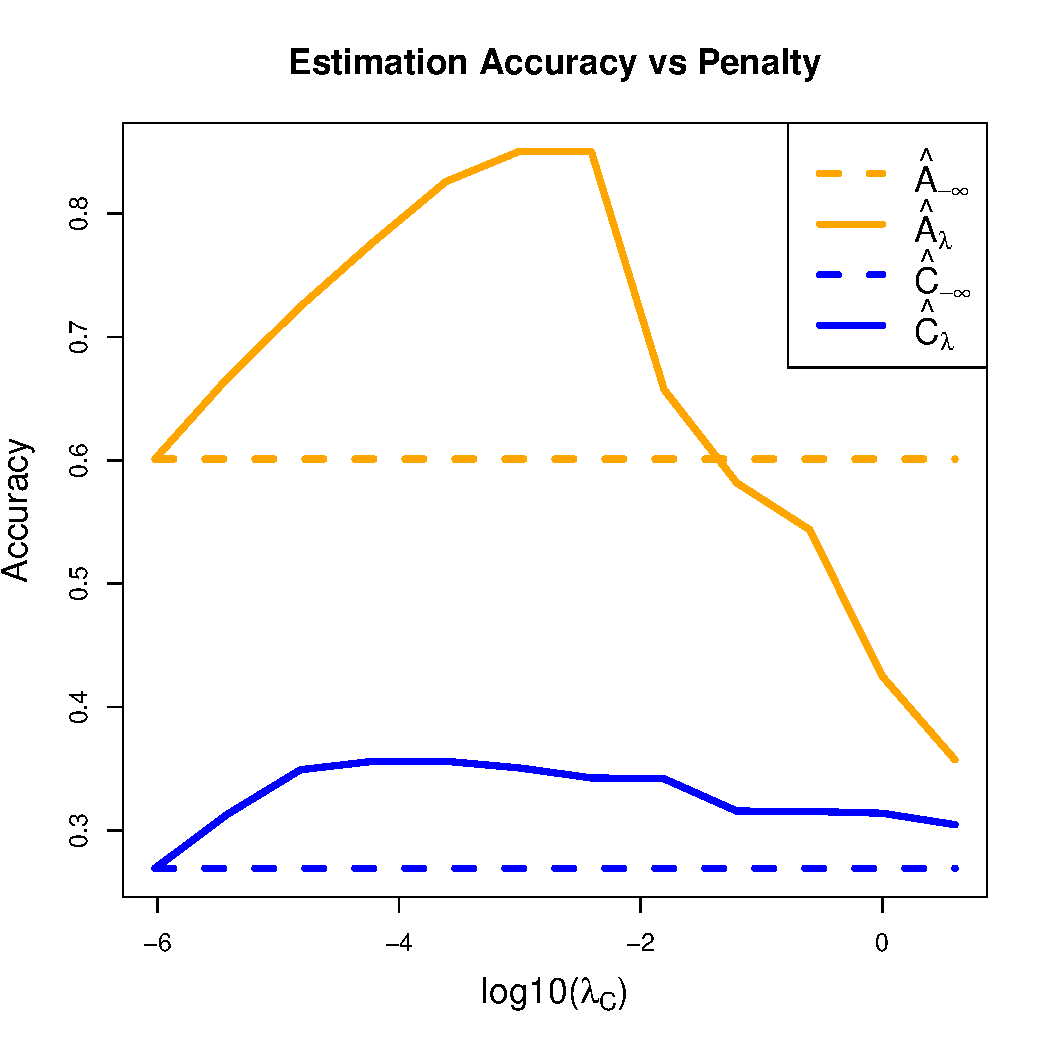
\includegraphics[scale=.43]{high-d-simulation.pdf}
}
\caption{$x$ axis is tuning parameter $\lambda_C$ under log scale and $y$ axis is the distance between truth and estimations; $\lambda_A$ is increasing proportionally with $\lambda_C$. One can see that in both the low dimensional and hight dimensional setting, estimation accuracies for $A$ and $C$ first increase then decrease as penalty increases.}
\label{fig:low-high-d-sim}
\end{figure}

\begin{figure}
\centering
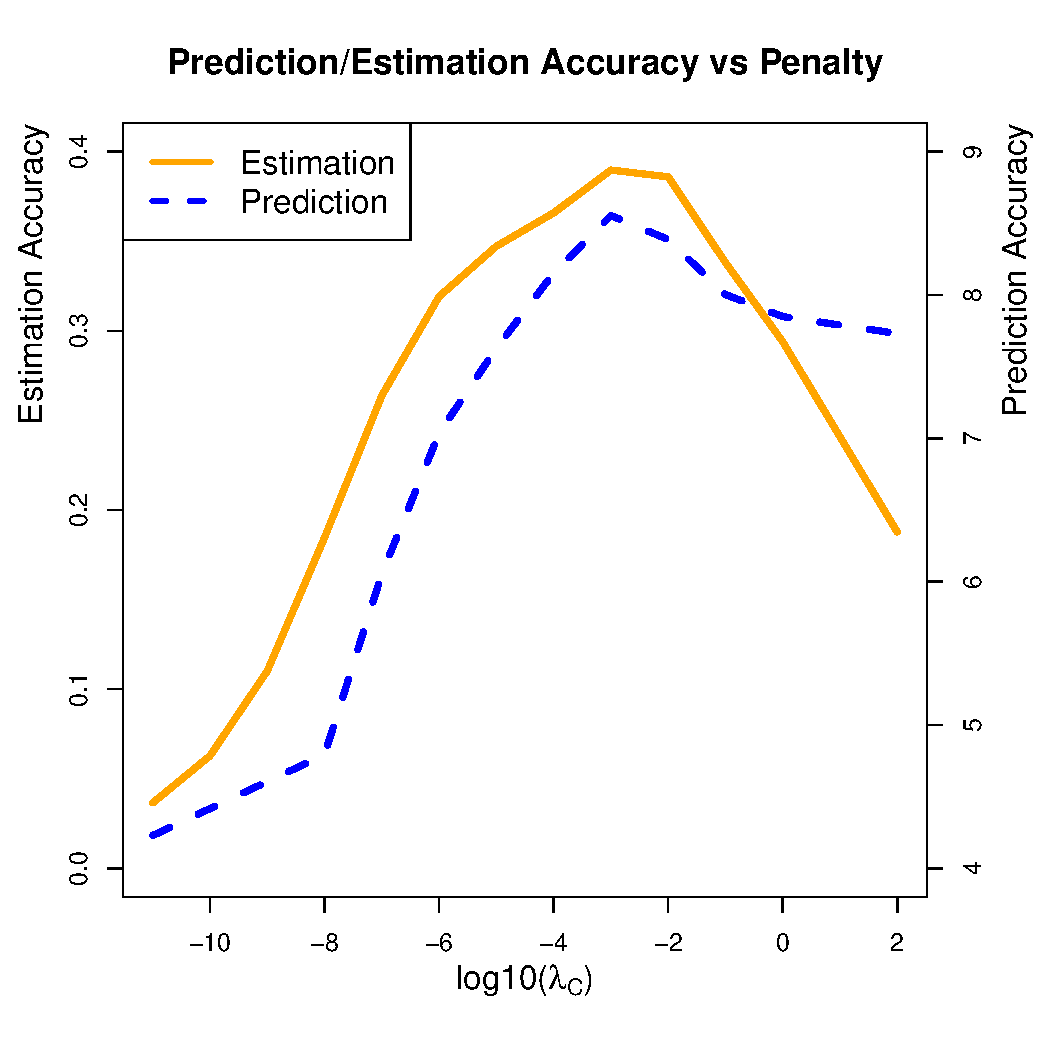
\includegraphics[scale=0.46]{est-pred-accuracy.pdf}
\captionof{figure}{Estimation and prediction accuracies. The $x$-axis represents the penalty size on a $\log$ scale. The $y$-axis represents the estimation and prediction accuracies. Note that the penalty which yields the most accurate estimation also gives the best prediction.}

\label{fig:estpredaccuracy}
\end{figure}

Both the standard LDS and \mrsid~  are applied to the simulation data. Estimation accuracies are plotted against penalty sizes in Figure \oldref{fig:low-high-d-sim}. From the plot, one sees that the prediction accuracy first improves, then drops when the penalties increase. \mrsid~  is also used for time series prediction, and the result is plotted in Figure \oldref{fig:estpredaccuracy}. The prediction accuracy peaks when the penalty coefficients $\lambda_A$ and $\lambda_C$ are around $10^{-3}$. This makes sense, as the same $(\lambda_A,\lambda_C)$ pair also gives the best estimations of $A$ and $C$, as seen in Figure \oldref{fig:low-high-d-sim}. The latter observation provides us a way to pick tuning parameters in real applications: one can use a collection of tuning parameter pairs $(\lambda_A,\lambda_C)$ for estimations (with train data) and subsequently for predictions (with test data). The pair that gives the most accurate out-of-sample predictions is picked. This trick is used in Section \oldref{sec:application}.

\section{Application}
\label{sec:application}

\subsection{Data and Motivation}
\mrsid~is applied to two datasets in this section: the Kirby 21 data and the Human Connectome Project (HCP) data.

The Kirby 21 data were acquired from the FM Kirby Research Center at the Kennedy Krieger Institute, an affiliate of Johns Hopkins University \citep{landman2011multi}. Twenty-one healthy volunteers with no history of neurological disease each underwent two separate resting state fMRI sessions on the same scanner. The data are preprocessed with FSL, a comprehensive library of analysis tools for fMRI, MRI, and DTI brain imaging data \citep{smith2004advances}. Specifically, FSL is used for spatial smoothing with a Gaussian kernel. Then \mrsid~was applied on the smoothed data.  The number of scans was $T = 210$.

The Human Connectome Project (HCP) is a systematic effort to map macroscopic human brain circuits and their relationship to behavior in a large population of healthy adults \citep{van2013wu,moeller2010multiband,feinberg2010multiplexed}. All scans consist of 1,200 time points. A comprehensive introduction of the dataset is given by \cite{van2013wu}.

Extensive research has been done to analyze the above datasets. Methods such as PCA and ICA (Independent Component Analysis) have been applied to obtain spatial decompositions of the brain, as well as the functional connectivity among the decomposed regions.  Thus, for our first application, we applied \mrsid~to the Kirby 21 data with the intent of obtaining both a spatial decomposition graph and a connectivity graph. As a second application, \mrsid~ was applied to the HCP data to predict brain activities. For both datasets, the motor cortex, which contains $p=7396$ voxels, is analyzed instead of the whole brain.
\subsection{Results}
\mrsid~is first applied to two subjects (four scans) from the Kirby 21 dataset. To pick the optimal penalty size, different values of  $\lambda_A = \lambda_C$ were attempted. Their values range from $10^{-10}$ to $10^{4}$. Then the estimated models with each combination were used to make predictions. We use the value of $10^{-5}$, as it gives the most accurate out-of-sample predictions. To determine the number of latent states, $d$, the profile likelihood method proposed by Zhu et al. \citep{zhu2006automatic} is utilized. The method assumes the eigenvalues of the data matrix follow a Gaussian mixture, and uses profile likelihood to pick the optimal number of latent states. Apply the method to all four scans, the numbers of latent states are 11, 6, 14 and 15 respectively. Their average, $d=11$, is used.

First, let's look at the estimations of $A$ matrix. Let $A_{12}$ stand for the estimated $A$ matrix for the second scan of subject one. Similar logic applies to the $A_{11}, A_{21}$, $A_{22}$, and $C$ matrices. These matrices contain subject-specific information. $4$ matrices leads to $6$ unique pairs. Intuitively, the pair $(A_{11},A_{12})$ and $(A_{21},A_{22})$ should have the highest similarity, as each comes from two scans of the same subject. This idea is validated by Table \oldref{tab:similarity}, which summarize similarities among the  $4$ matrices. The distance measure in Eq.~\ref{eq:distance} was used. The Amari error \citep{amari1996new}, which is another permutation-invariant measure of similarity, is also provided. A smaller $d(A,B)$ or Amari error means higher similarity.
\begin{table}
\centering
\captionof{table}{Similarities Among Estimated $A$ Matrices}
\label{tab:similarity}
\begin{tabular}{c|cccc}
\hline
$d_{A,B}$ & $A_{11}$&$A_{12}$ & $A_{21}$&$A_{22}$ \\
\hline
$A_{11}$ & $0$ &  &  &\\
$A_{12}$ & $\mathbf{0.076(0.88)}$& $0$ & &\\
$A_{21}$ & $0.105(1.05)$ & $0.095(1.08)$  & $0$ &\\
$A_{22}$ & $0.095(1.02)$ & $0.095(1.09)$ & $\mathbf{0.085(0.98)}$ & $0$ \\
\hline
\end{tabular}
\end{table}

Next, let's look at the $C$ matrices. 3D renderings of the columns of $C_{11}$ are shown in Figure \oldref{fig:3d}. The 3D regions in the plot are comparable to existing parcellations of the motor cortex. As an example, the blue region in Figure \oldref{fig:3d} accurately matches the dorsomedial (DM) parcel of the five-region parcellation proposed by Nebel MB et al. \citep{nebel2014disruption}.

\begin{center}
\[
\begin{array}{lll}
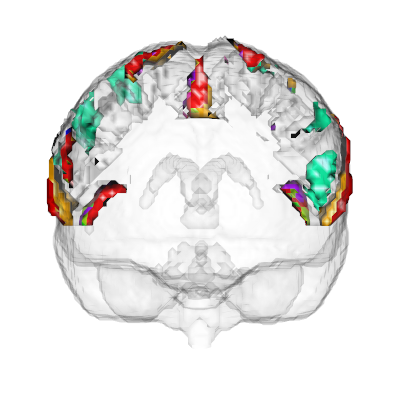
\includegraphics[scale = 0.18]{view1.png} & 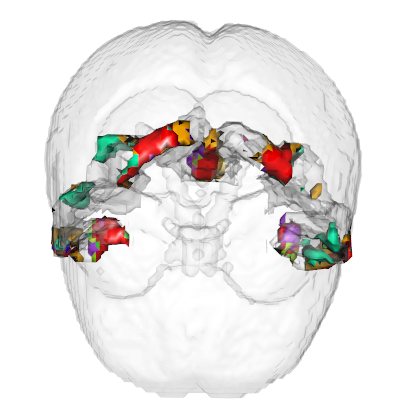
\includegraphics[scale = 0.165]{view2.png} & 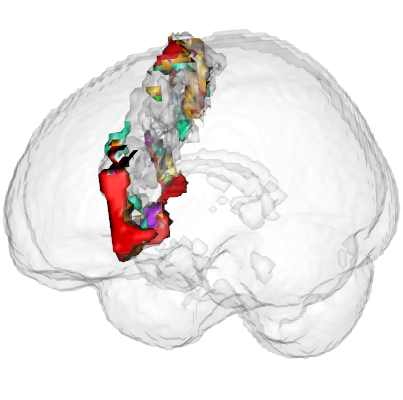
\includegraphics[scale = 0.165]{view3.png}

\end{array}
\]
\captionof{figure}{3D rendering of columns of matrix $C_{11}$: estimation for the first scan of subject one.}
\label{fig:3d}
\end{center}

Matrix $A$ and $C$ have natural interpretation here. Each $\by_t$ is a snapshot of brain activity at time $t$. The columns of $C$ are interpreted as time-invariant brain ``point spread functions''. At each time point, the observed brain image, $\by_t$, is a linear mixture of latent co-assemblies of neural activity  $\bx_t$. Matrix $A$ describes how $\bx_t$ evolves over time. $A$ is a directed graph if one treats each neural assembly as a vertex. Each neural assembly is spatially smooth, and connectivity across them is empirically sparse. This naturally fits into the sparsity and smoothness assumptions of \mrsid.

To summarize, \mrsid~ gives a spatial decomposition of the motor cortex, as well as the sparse connectivity among the decomposed regions. The connectivity graph contains subject-specific information and can correctly group scans by subject. The decomposed regions are spatially smooth and are comparable to existing parcellations of the motor cortex.

As a second application, \mrsid~is applied to the HCP data to predict brain signals.
Using the profile likelihood method, $d=149$ is picked. HCP data has $T=1200$ time points. The first $N = 1000$ (about $80\%$) were used as training data, while the rest were used as out-of-sample test data.
\mrsid~was used to predict brain activity from the training data. As a comparison, the SVD method to initialize \mrsid~is also attempted. Both methods were first used for parameter estimations, then the estimated parameters were fed into equations \ref{eq:model0} to make $k$-step ahead predictions. Pseudocode for $k$-step ahead predictions is given in the Appendix.

The prediction accuracies are shown in Figure \oldref{fig:predaccy}. One can see that the \mrsid~algorithm gives significantly more accurate predictions for the first 150 steps compared to the SVD method. Considering the fact that the SVD method is used to initialize \mrsid, this observation shows that \mrsid~makes real improvement on top of the SVD method. Another observation is that the performance of \mrsid~suffers when one predicts too far into the future ($>150$ steps). This is because the prediction errors from each step will accumulate, yielding deteriorating accuracies as the number of steps increase.
%\begin{figure}
%\centering
%\subfigure[]{
%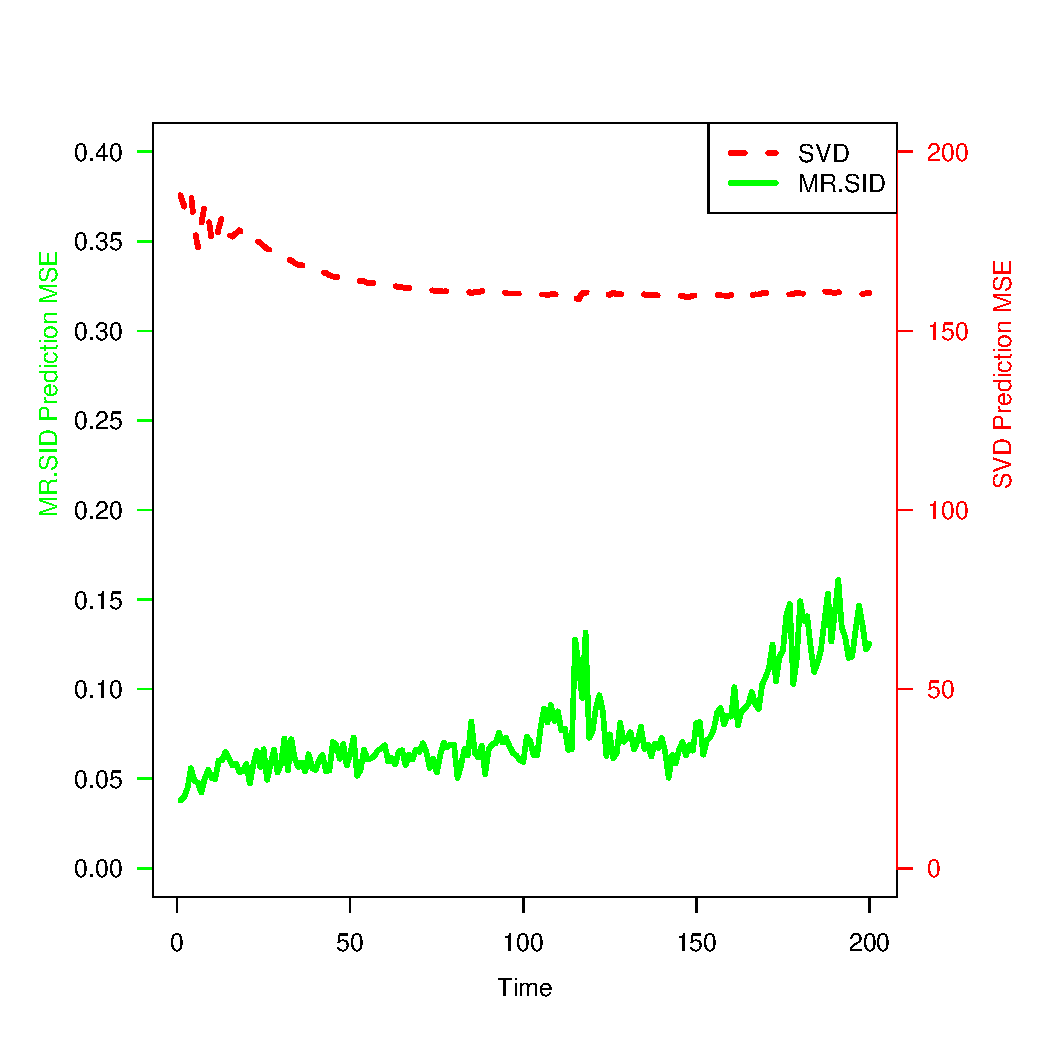
\includegraphics[scale=0.45]{hcp_pred_accy.pdf}
%}
%\subfigure[]{
%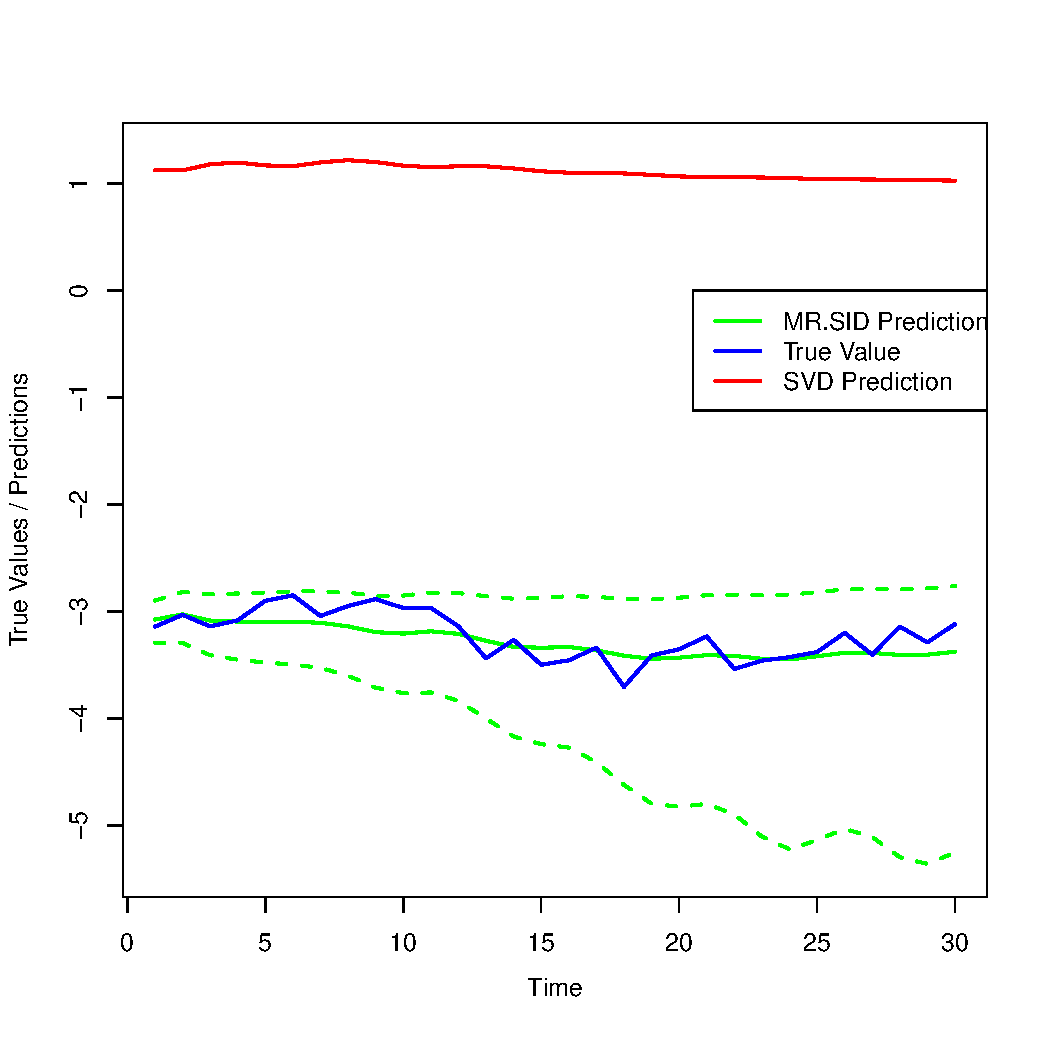
\includegraphics[scale=0.4]{newSampleTS.pdf}
%}
%\subfigure[]{
%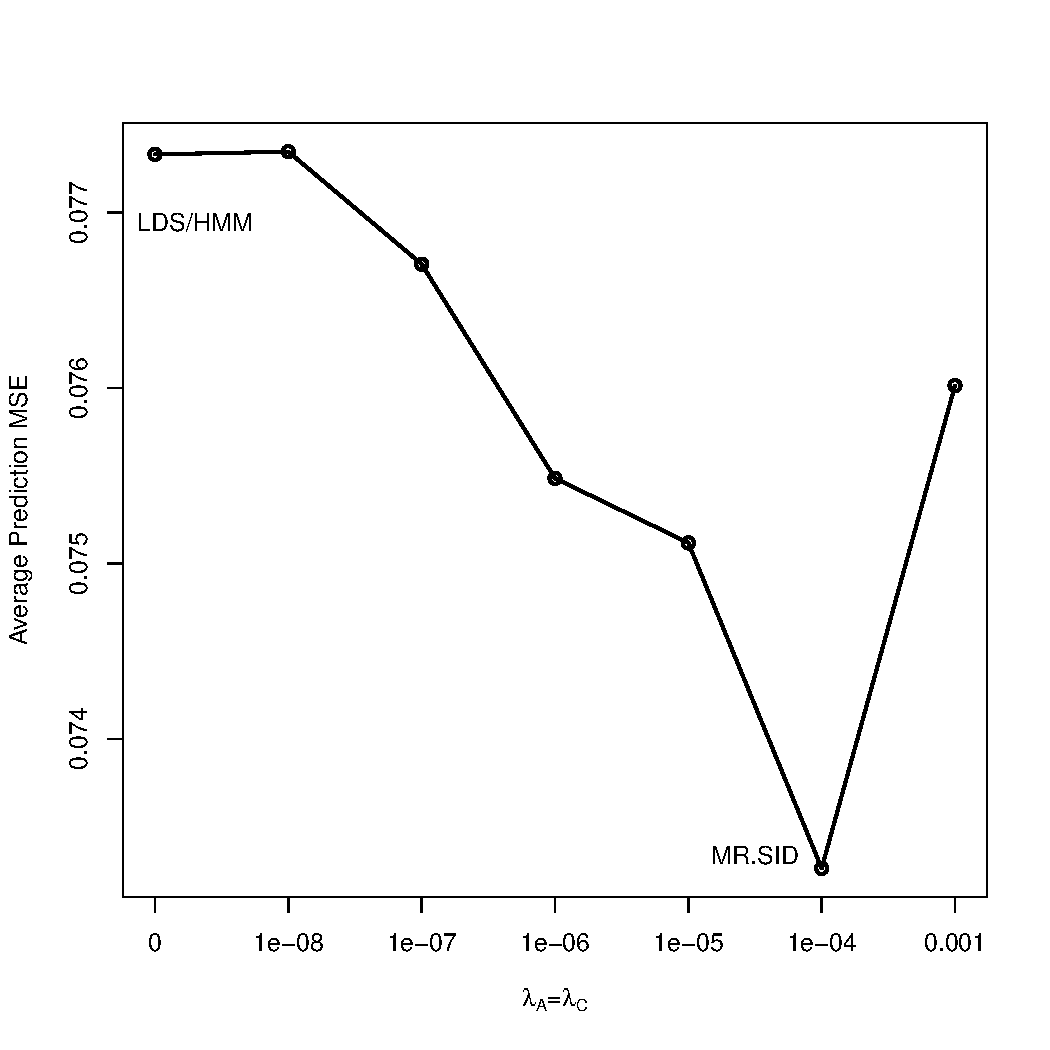
\includegraphics[scale=0.4]{plds_lds_pred_comparison.pdf}
%}
%\vspace*{-5mm}
%\captionof{figure}{Comparison of prediction accuracies on HCP data.
%\emph{(a):} Accuracies of \mrsid~and SVD predictions over time, with accuracy measured through mean squared error (MSE).
%\emph{(b):} Sample time series plot. The dotted green curve represents the $60\%$ confidence band given by the \mrsid~model. The true time series consists of averaged signals from a subsample of voxels. The predictions were also averaged over the same subsample. The confidence band was estimated based on the covariance matrix of these voxels. A subsample of 20 voxels were selected for this experiment, to avoid the calculation of large covariance matrices. All values were log-scaled for plotting purposes.
%}
%\label{fig:predaccy}
%\end{figure}
\begin{figure}
\centering
\vspace*{-5mm}
\begin{tabular}{c}
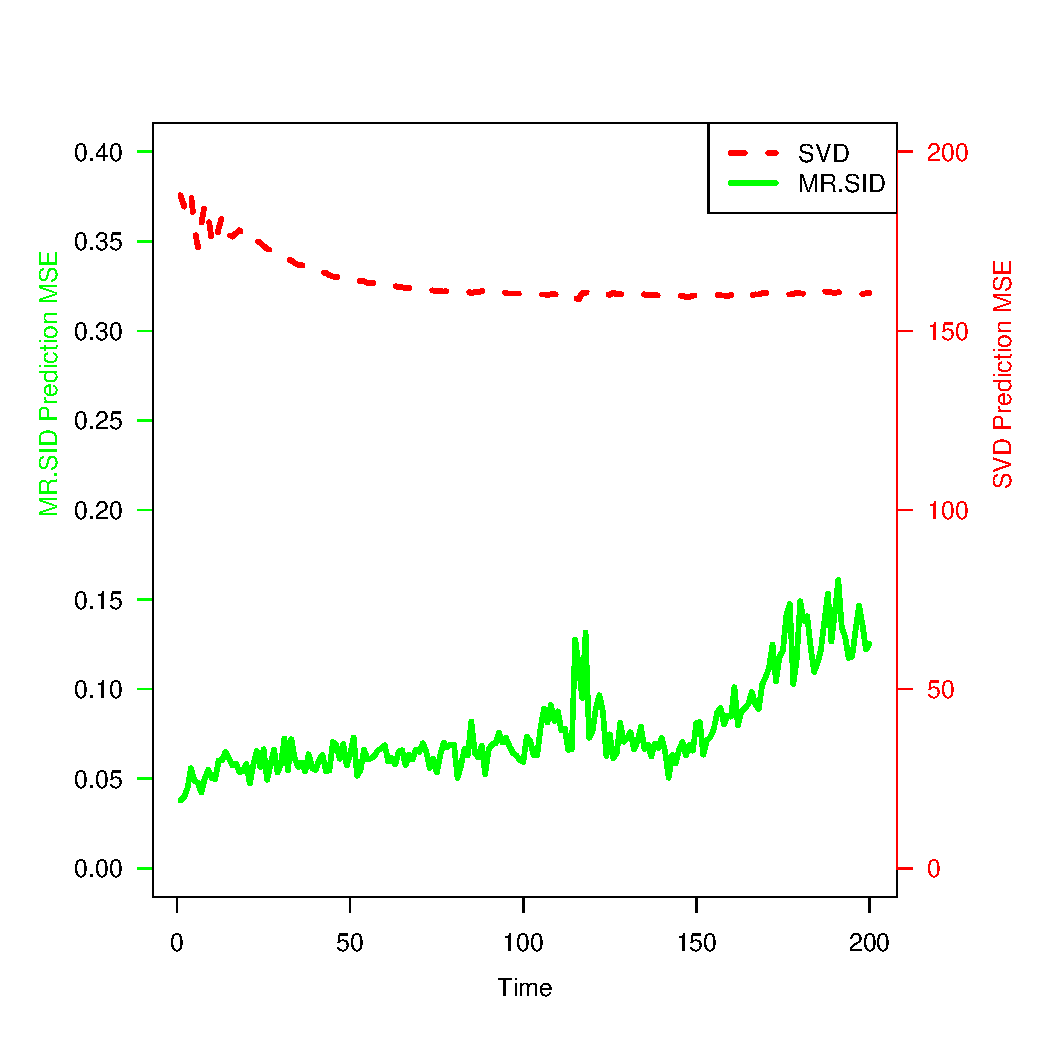
\includegraphics[scale=0.45]{hcp_pred_accy.pdf}\\
\vspace*{-5mm}
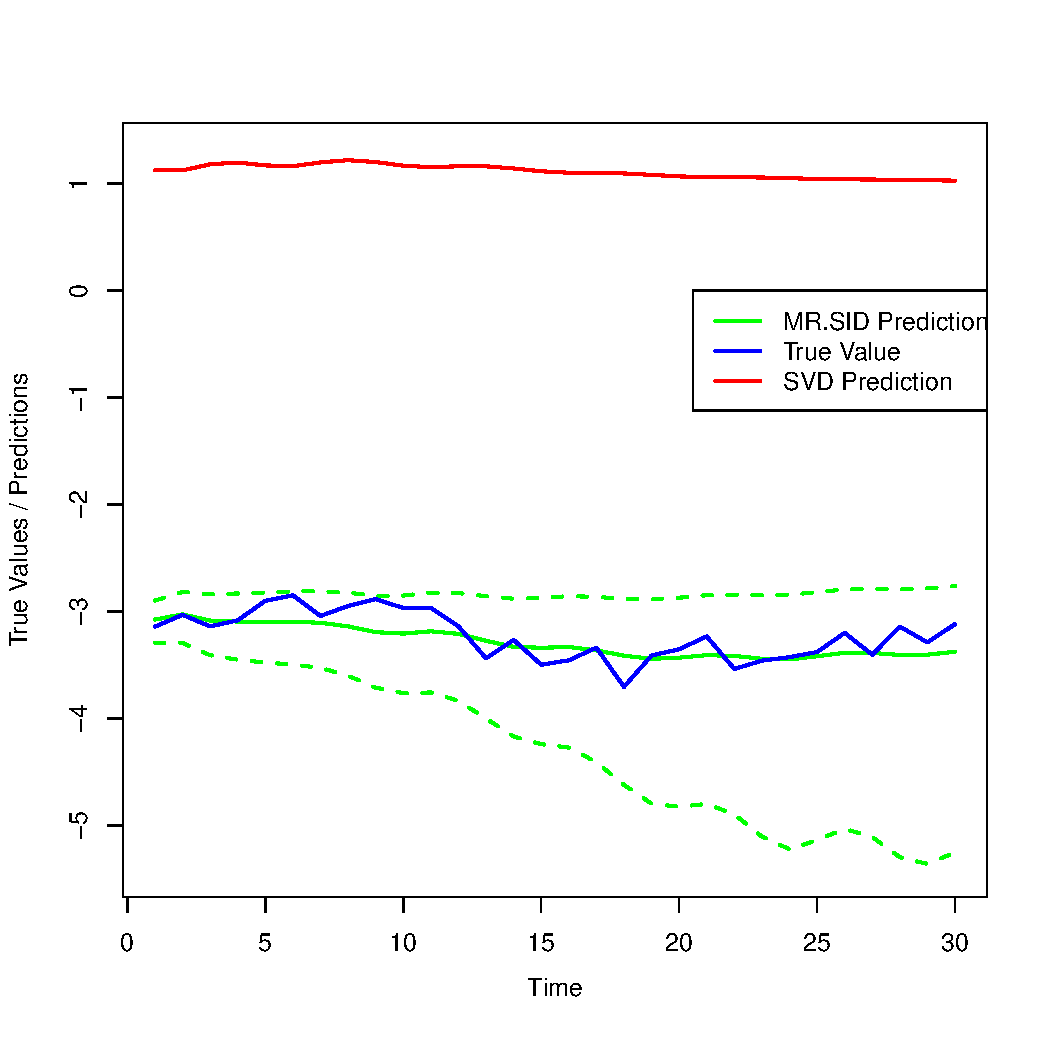
\includegraphics[scale=0.4]{newSampleTS.pdf}\\
\vspace*{-5mm}
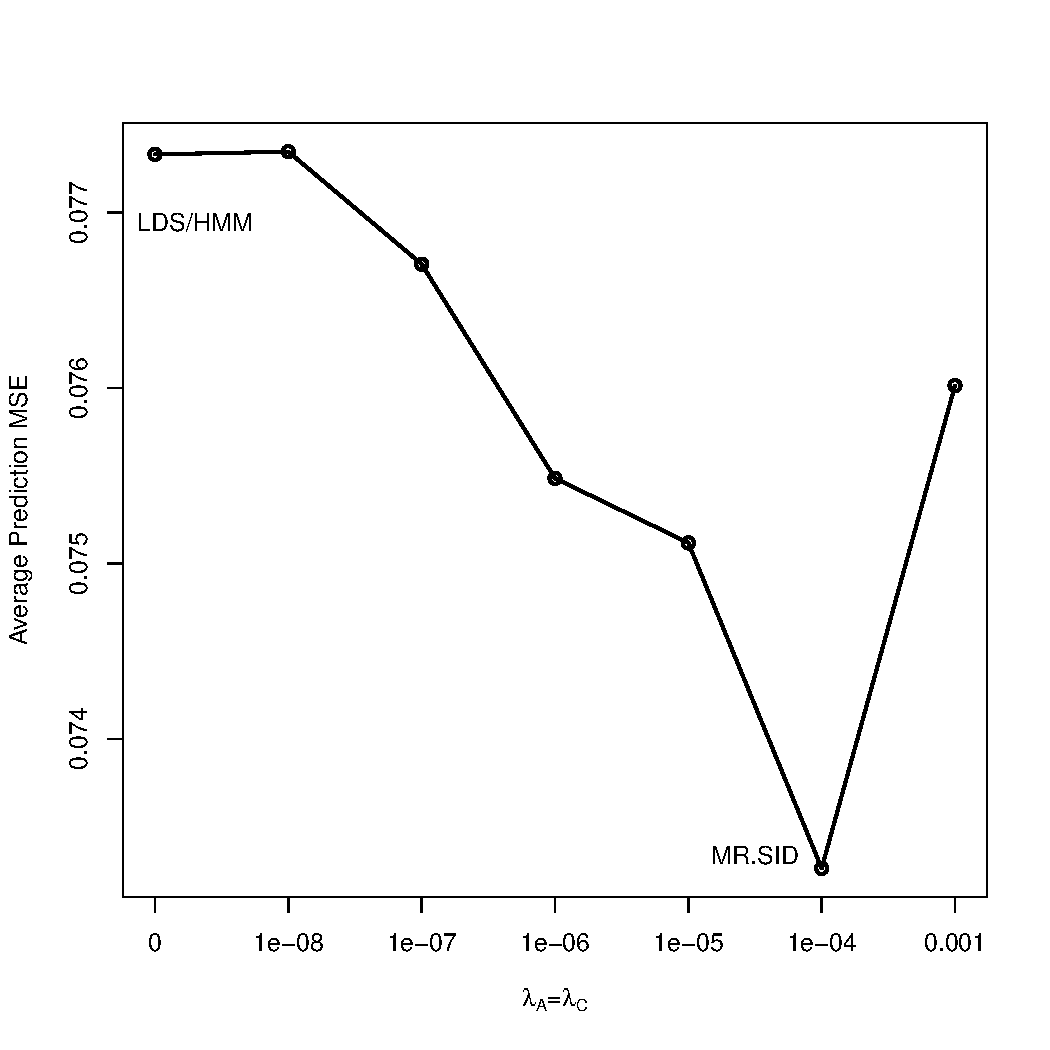
\includegraphics[scale=0.4]{plds_lds_pred_comparison.pdf}
\end{tabular}
\captionof{figure}{Comparison of prediction accuracies on HCP data.
\emph{(1):} Accuracies of \mrsid~and SVD predictions over time, with accuracy measured as mean squared error (MSE).
\emph{(2):} Sample time series plot. The dotted green curve represents the $60\%$ confidence band given by the \mrsid. The true time series are averaged signals from a subsample of 20 voxels. Predictions were averaged over the same subsample. The confidence band was estimated via the covariance matrix of these voxels. Values were log-scaled for plotting.
\emph{(3):} Comparison of prediction accuracy of LDS/HMM and \mrsid: \mrsid~gives better prediction than LDS/HMM, which is a special case of \mrsid.
}
\label{fig:predaccy}
\end{figure}
A sample plot of the true time series and predicted values are shown in Figure \oldref{fig:predaccy}. We see that \mrsid~gives more accurate predictions, and the true signal lies in the confidence band given by the \mrsid~model. Note that the confidence band is wider for predictions farther into the future, which is a result of the accumulated errors discussed previously.
\section{Discussion}
We have taken a first step towards the modeling and estimation of high-dimensional time-series data. The proposed method balances both statistical and computational considerations.  Indeed, much like the Kalman Filter-Smoother for modeling time-series data, and the Baum-Welch algorithm for system identification act as ``primitives'' for time-series data analysis, \mrsid~can act as a primitive for similar time-series analysis when the dimensionality is significantly larger than the number of time steps.  Via simulations we demonstrated the efficacy of our methods.  Then, by applying the proposed approach to fMRI scans of the motor cortex of healthy adults, we identified limited sub-regions (networks) from the motor cortex.

In the future, this work could be extended in two important directions. First, assumptions on the covariance structures in the observation equation could be generalized. Prior knowledge could be incorporated into the covariance matrix $R$ \citep{allen2014generalized}. The idea is that $R$ should be general enough to be flexible, but sufficiently restricted to make the model useful. Many other methods, e.g. those that use tridiagonal and upper triangular matrices, could also be considered. Mohammad et al. have discussed the impact of autocorrelation on functional connectivity, which also provides some direction for extension \citep{arbabshirani2014impact}.

Finally, the work can also be extended on the application side. Currently, only data from a few subjects have been analyzed. As a next step, the model can be extended to a group version and be used to analyze more subjects. In addition, the $A$ matrix estimated by \mrsid~could potentially be used as a measure of fMRI scan reproducibility.

\section*{Acknowledgements}
This work is graciously supported by the Defense Advanced Research Projects Agency (DARPA) SIMPLEX program through SPAWAR contract N66001-15-C-4041 and DARPA GRAPHS N66001-14-1-4028.

\bibliographystyle{Chicago}
\bibliography{reference}

\end{document}

%%
